\documentclass[tikz,border=4pt]{standalone}
\usepackage{amsmath}
\usepackage{xcolor}
\usepackage{tikz}
\usepackage{pgfplots}
\pgfplotsset{compat=1.18}

\definecolor{caraprimary}{RGB}{30,60,120}
\definecolor{caraaccent}{RGB}{200,80,60}

\begin{document}
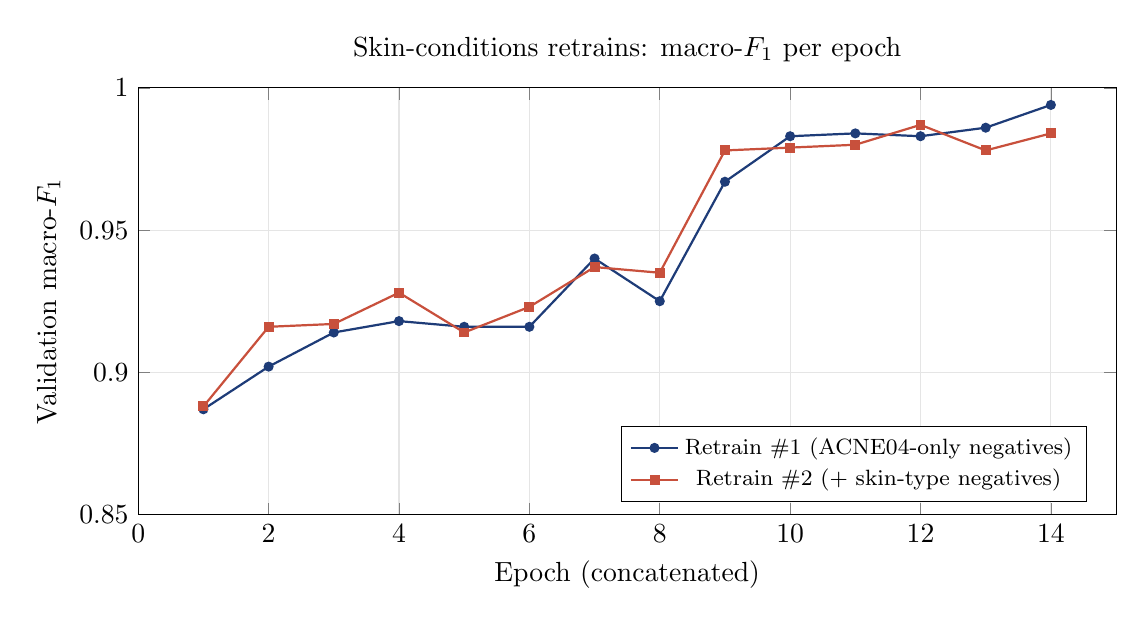
\begin{tikzpicture}
\begin{axis}[
    width=14cm, height=7cm,
    xlabel={Epoch (concatenated)},
    ylabel={Validation macro-\(F_1\)},
    ymin=0.85, ymax=1.00,
    xmin=0, xmax=15,
    grid=both, grid style={gray!20},
    legend pos=south east,
    legend style={font=\footnotesize},
    title={Skin-conditions retrains: macro-\(F_1\) per epoch}]
\addplot[thick, color=caraprimary, mark=*, mark size=1.4pt] coordinates {
    (1,0.887)(2,0.902)(3,0.914)(4,0.918)(5,0.916)(6,0.916)(7,0.940)(8,0.925)
    (9,0.967)(10,0.983)(11,0.984)(12,0.983)(13,0.986)(14,0.994)
};
\addlegendentry{Retrain \#1 (ACNE04-only negatives)}
\addplot[thick, color=caraaccent, mark=square*, mark size=1.4pt] coordinates {
    (1,0.888)(2,0.916)(3,0.917)(4,0.928)(5,0.914)(6,0.923)(7,0.937)(8,0.935)
    (9,0.978)(10,0.979)(11,0.980)(12,0.987)(13,0.978)(14,0.984)
};
\addlegendentry{Retrain \#2 (\(+\) skin-type negatives)}
\end{axis}
\end{tikzpicture}
\end{document}
